
\chapter{Writing a TANGO client using TANGO APIs}


\section{Introduction}

\noindent TANGO devices and database are implemented using the TANGO
device server model. To access them the user has the CORBA interface
e.g. command\_inout(), write\_attributes() etc. defined by the idl
file. These methods are very low-level and assume a good working knowledge
of CORBA. In order to simplify this access, high-level api has been
implemented which hides all CORBA aspects of TANGO. In addition the
api hides details like how to connect to a device via the database,
how to reconnect after a device has been restarted, how to correctly
pack and unpack attributes and so on by implementing these in a manner
transparent to the user. The api provides a unified error handling
for all TANGO and CORBA errors. Unlike the CORBA C++ bindings the
TANGO api supports native C++ data types e.g. strings and vectors.

This chapter describes how to use these API's. It is not a reference
guide. Reference documentation is available as Web pages in the \href{http://www.tango-controls.org}{Tango Web site}


\section{\noindent Getting Started}

Refer to the chapter \textquotedbl{}Getting Started\textquotedbl{}
for an example on getting start with the C++ or Java api.


\section{\noindent Basic Philosophy}

\noindent The basic philosophy is to have high level classes to deal
with Tango devices. To communicate with Tango device, uses the \textbf{DeviceProxy\index{DeviceProxy}}
class. To send/receive data to/from Tango device, uses the \textbf{DeviceData\index{DeviceData},
DeviceAttribute\index{DeviceAttribute}} or \textbf{DevicePipe}\index{DevicePipe}
classes. To communicate with a group of devices, use the \textbf{Group\index{Group}}
class. If you are interested only in some attributes provided by a
Tango device, uses the \textbf{AttributeProxy\index{AttributeProxy}}
class. Even if the Tango database is implemented as any other devices
(and therefore accessible with one instance of a DeviceProxy class),
specific high level classes have been developped to query it. Uses
the \textbf{Database}\index{Database}, \textbf{DbDevice}\index{DbDevice},
\textbf{DbClass}\index{DbClass}, \textbf{DbServer\index{DbServer}}
or \textbf{DbData\index{DbData}} classes when interfacing the Tango
database. Callback for asynchronous requests or events are implemented
via a \textbf{CallBack\index{CallBack}} class. An utility class called
\textbf{ApiUtil\index{ApiUtil}} is also available.


\section{Data types}

The definition of the basic data type you can transfert using Tango
is:

\vspace{0.3cm}


\begin{center}
\begin{longtable}{|c|c|}
\hline 
Tango type name & C++ equivalent type\tabularnewline
\hline 
\hline 
DevBoolean & boolean\tabularnewline
\hline 
DevShort & short\tabularnewline
\hline 
DevEnum & enumeration (only for attribute / See chapter on advanced features)\tabularnewline
\hline 
DevLong & int (always 32 bits data)\tabularnewline
\hline 
DevLong64 & long long on 32 bits chip or long on 64 bits chip\tabularnewline
 & always 64 bits data\tabularnewline
\hline 
DevFloat & float\tabularnewline
\hline 
DevDouble & double\tabularnewline
\hline 
DevString & char {*}\tabularnewline
\hline 
DevEncoded & structure with 2 fields: a string and an array of unsigned char\tabularnewline
\hline 
DevUChar & unsigned char\tabularnewline
\hline 
DevUShort & unsigned short\tabularnewline
\hline 
DevULong & unsigned int (always 32 bits data)\tabularnewline
\hline 
DevULong64 & unsigned long long on 32 bits chip or unsigned long on 64 bits chip\tabularnewline
 & always 64 bits data\tabularnewline
\hline 
DevState & Tango specific data type\tabularnewline
\hline 
\end{longtable}
\par\end{center}

\vspace{0.3cm}


Using commands, you are able to transfert all these data types, array
of these basic types and two other Tango specific data types called
DevVarLongStringArray and DevVarDoubleStringArray. See chapter \ref{Data exchange}
to get details about them. You are also able to create attributes
using any of these basic data types to transfer data between clients
and servers.


\section{Request model}
\label{sec:Request-model}

For the most important API remote calls (command\_inout, read\_attribute(s)
and write\_attribute(s)), Tango supports two kind of requests which
are the synchronous model and the asynchronous model. Synchronous\index{synchronous}
model means that the client wait (and is blocked) for the server to
send an answer. Asynchronous\index{asynchronous} model means that
the client does not wait for the server to send an answer. The client
sends the request and immediately returns allowing the CPU to do anything
else (like updating a graphical user interface). Device pipe\index{pipe}
supports only the synchronous model. Within Tango, there are two ways
to retrieve the server answer when using asynchronous model. They
are:
\begin{enumerate}
\item The polling\index{polling} mode
\item The callback\index{callback} mode
\end{enumerate}
In polling mode, the client executes a specific call to check if the
answer is arrived. If this is not the case, an exception is thrown.
If the reply is there, it is returned to the caller and if the reply
was an exception, it is re-thrown. There are two calls to check if
the reply is arrived:
\begin{itemize}
\item Call which does not wait before the server answer is returned to the
caller.
\item Call which wait with timeout before returning the server answer to
the caller (or throw the exception) if the answer is not arrived.
\end{itemize}
In callback model, the caller must supply a callback method which
will be executed when the command returns. They are two sub-modes:
\begin{enumerate}
\item The pull\index{pull} callback mode
\item The push\index{push} callback mode
\end{enumerate}
In the pull callback\index{callback} mode, the callback is triggered
if the server answer is arrived when the client decide it by calling
a \emph{synchronization} method (The client pull-out the answer).
In push mode, the callback is executed as soon as the reply arrives
in a separate thread (The server pushes the answer to the client).


\subsection{Synchronous model}

Synchronous access to Tango device are provided using the \emph{DeviceProxy}
or \emph{AttributeProxy} class. For the \emph{DeviceProxy} class,
the main synchronous call methods are :
\begin{itemize}
\item \emph{command\_inout()} to execute a Tango device command
\item \emph{read\_attribute()} or \emph{read\_attributes()} to read a Tango
device attribute(s)
\item \emph{write\_attribute()} or \emph{write\_attributes()} to write a
Tango device attribute(s)
\item \emph{write\_read\_attribute()} or \emph{write\_read\_attributes()}
to write then read Tango device attribute(s)
\item \emph{read\_pipe()} to read a Tango device pipe
\item \emph{write\_pipe()} to write a Tango device pipe
\item \emph{write\_read\_pipe()} to write then read Tango device pipe
\end{itemize}
For commands, data are send/received to/from device using the \emph{DeviceData}
class. For attributes, data are send/received to/from device attribute
using the \emph{DeviceAttribute} class. For pipes, data are send/receive
to/from device pipe using the \emph{DevicePipe\index{DevicePipe}}
and \emph{DevicePipeBlob\index{DevicePipeBlob}} classes.

In some cases, only attributes provided by a Tango device are interesting
for the application. You can use the \emph{AttributeProxy} class.
Its main synchronous methods are :
\begin{itemize}
\item \emph{read()} to read the attribute value
\item \emph{write()} to write the attribute value
\item \emph{write\_read()} to write then read the attribute value
\end{itemize}
Data are transmitted using the \emph{DeviceAttribute} class.


\subsection{Asynchronous model}

Asynchronous access to Tango device are provided using \emph{DeviceProxy}
or \emph{AttributeProxy, CallBack} and \emph{ApiUtil} classes methods.
The main asynchronous call methods and used classes are :
\begin{itemize}
\item To execute a command on a device

\begin{itemize}
\item \emph{DeviceProxy::command\_inout\_asynch()} and \emph{DeviceProxy::command\_inout\_reply()}
in polling model.
\item \emph{DeviceProxy::command\_inout\_asynch()}, \emph{DeviceProxy::get\_asynch\_replies()}
and \emph{CallBack} class in callback pull model
\item \emph{DeviceProxy::command\_inout\_asynch()}, \emph{ApiUtil::set\_asynch\_cb\_sub\_model()}
and \emph{CallBack} class in callback push model
\end{itemize}
\item To read a device attribute 

\begin{itemize}
\item \emph{DeviceProxy::read\_attribute\_asynch()} and \emph{DeviceProxy::read\_attribute\_reply()}
in polling model
\item \emph{DeviceProxy::read\_attribute\_asynch()}, \emph{DeviceProxy::get\_asynch\_replies()}
and \emph{CallBack} class in callback pull model.
\item \emph{DeviceProxy::read\_attribute\_asynch()}, \emph{ApiUtil::set\_asynch\_cb\_sub\_model()}
and \emph{CallBack} class in callback push model
\end{itemize}
\item To write a device attribute

\begin{itemize}
\item \emph{DeviceProxy::write\_attribute\_asynch()} in polling model
\item \emph{DeviceProxy::write\_attribute\_asynch()} and \emph{CallBack}
class in callback pull model
\item \emph{DeviceProxy::write\_attribute\_asynch()}, \emph{ApiUtil::set\_asynch\_cb\_sub\_model()}
and \emph{CallBack} class in callback push model
\end{itemize}
\end{itemize}
For commands, data are send/received to/from device using the \emph{DeviceData}
class. For attributes, data are send/received to/from device attribute
using the \emph{DeviceAttribute} class. It is also possible to generate
asynchronous request(s) using the \emph{AttributeProxy\index{AttributeProxy}}
class following the same schema than above. Methods to use are :
\begin{itemize}
\item \emph{read\_asynch(}) and \emph{read\_reply()} to asynchronously read
the attribute value
\item \emph{write\_asynch()} and \emph{write\_reply()} to asynchronously
write the attribute value
\end{itemize}

\section{Events\index{event}}


\subsection{Introduction}

Events are a critical part of any distributed control system. Their
aim is to provide a communication mechanism which is fast and efficient. 

The standard CORBA communication paradigm is a synchronous or asynchronous
two-way call. In this paradigm the call is initiated by the client
who contacts the server. The server handles the client's request and
sends the answer to the client or throws an exception which the client
catches. This paradigm involves two calls to receive a single answer
and requires the client to be active in initiating the request. If
the client has a permanent interest in a value he is obliged to poll
the server for an update in a value every time. This is not efficient
in terms of network bandwidth nor in terms of client programming.

For clients who are permanently interested in values the event-driven
communication paradigm is a more efficient and natural way of programming.
In this paradigm the client registers her interest once in an event
(value). After that the server informs the client every time the event
has occurred. This paradigm avoids the client polling, frees it for
doing other things, is fast and makes efficient use of the network.

The rest of this chapter explains how the TANGO events are implemented
and the application programmer's interface.


\subsection{Event definition}

TANGO events represent an alternative channel for reading TANGO device
attributes\index{attribute}. Device attributes values are sent to
all subscribed clients when an event occurs. Events can be an attribute
value change, a change in the data quality or a periodically send
event. The clients continue receiving events as long as they stay
subscribed. Most of the time, the device server polling thread detects
the event and then pushes the device attribute value to all clients.
Nevertheless, in some cases, the delay introduced by the polling thread
in the event propagation is detrimental. For such cases, some API
calls directly push the event. Until TANGO release 8, the omniNotify\index{omniNotify}
implementation of the CORBA Notification service\index{Notification Service}
was used to dispatch events. Starting with TANGO 8, this CORBA Notification
service has been replaced by the ZMQ\index{ZMQ} library which implements
a Publish/Subscribe communication model well adapted to TANGO events
communication.


\subsection{Event types}

The following eight event types have been implemented in TANGO :
\begin{enumerate}
\item \textbf{change\index{change}} - an event is triggered and the attribute
value is sent when the attribute value changes significantly. The
exact meaning of significant is device attribute dependent. For analog
and digital values this is a delta fixed per attribute, for string
values this is any non-zero change i.e. if the new attribute value
is not equal to the previous attribute value. The delta can either
be specified as a relative or absolute change. The delta is the same
for all clients unless a filter is specified (see below). To easily
write applications using the change event, it is also triggered in
the following case :

\begin{enumerate}
\item When a spectrum or image attribute size changes.
\item At event subscription time
\item When the polling thread receives an exception during attribute reading
\item When the polling thread detects that the attribute quality factor
has changed.
\item The first good reading of the attribute after the polling thread has
received exception when trying to read the attribute
\item The first time the polling thread detects that the attribute quality
factor has changed from INVALID to something else
\item When a change event is pushed manually from the device server code.
(\emph{DeviceImpl::push\_change\_event()}).
\item By the methods Attribute::set\_quality() and Attribute::set\_value\_date\_quality()
if a client has subscribed to the change event on the attribute. This
has been implemented for cases where the delay introduced by the polling
thread in the event propagation is not authorized.
\end{enumerate}
\item \textbf{periodic\index{periodic}} - an event is sent at a fixed periodic
interval. The frequency of this event is determined by the \emph{event\_period}
property of the attribute and the polling frequency. The polling frequency
determines the highest frequency at which the attribute is read. The
event\_period determines the highest frequency at which the periodic
event is sent. Note if the event\_period is not an integral number
of the polling period there will be a beating of the two frequencies%
\footnote{note: the polling is not synchronized is currently not synchronized
on the hour%
}. Clients can reduce the frequency at which they receive periodic
events by specifying a filter on the periodic event counter. 
\item \textbf{archive\index{archive}} - an event is sent if one of the
archiving conditions is satisfied. Archiving conditions are defined
via properties in the database. These can be a mixture of delta\_change
and periodic. Archive events can be send from the polling thread or
can be manually pushed from the device server code (\emph{DeviceImpl::push\_archive\_event()}).
\item \textbf{attribute configuration} - an event is sent if the attribute
configuration is changed.
\item \textbf{data ready} - This event is sent when coded by the device
server programmer who uses a specific method of one of the Tango device
server class to fire the event (\emph{DeviceImpl::push\_data\_ready\_event()}).
The rule of this event is to inform a client that it is now possible
to read an attribute. This could be useful in case of attribute with
many data.
\item \textbf{user} - The criteria and configuration of these user events
are managed by the device server programmer who uses a specific method
of one of the Tango device server class to fire the event (\emph{DeviceImpl::push\_event()}).
\item \textbf{device interface change} - This event is sent when the device
interface changes. Using Tango, it is possible to dynamically add/remove
attribute/command to a device. This event is the way to inform client(s)
that attribute/command has been added/removed from a device. Note
that this type of event is attached to a device and not to one attribute
(like all other event types). This event is triggered in the following
case :

\begin{enumerate}
\item A dynamic attribute or command is added or removed. The event is sent
after a small delay (50 mS) in order to eliminate the risk of events
storm in case several attributes/commands are added/removed in a loop 
\item At the end of admin device RestartServer or DevRestart command
\item After a re-connection due to a device server restart. Because the
device interface is not memorized, the event is sent even if it is
highly possible that the device interface has not changed. A flag
in the data propagated with the event inform listening applications
that the device interface change is not guaranteed. 
\item At event re-connection time. This case is similar to the previous
one (device interface change not guaranteed)
\end{enumerate}
\item \textbf{pipe} - This is the kind of event which has to be used when
the user want to push data through a pipe. This kind of event is only
sent by the user code by using a specific method (\emph{DeviceImpl::push\_pipe\_event()}).
There is no way to ask the Tango kernel to automatically push this
kind of event.
\end{enumerate}
The first three above events are automatically generated by the TANGO
library or fired by the user code. Events number 4 and 7 are only
automatically sent by the library and events 5, 6 and 8 are fired
only by the user code.


\subsection{Event filtering (Removed in Tango release 8 and above)}

Please, note that this feature is available only for Tango releases
older than Tango 8. The CORBA Notification Service allows event filtering.
This means that a client can ask the Notification Service to send
the event only if some filter is evaluated to true. Within the Tango
control system, some pre-defined fields can be used as filter. These
fields depend on the event type.

\vspace{0.3cm}


\begin{center}
\begin{longtable}{|c|c|c|c|}
\hline 
Event type & Filterable field name & Filterable field value & type\tabularnewline
\hline 
\hline 
 & delta\_change\_rel & Relative change (in \%) since last event & double\tabularnewline
\cline{2-4} 
\multicolumn{1}{|c|}{} & delta\_change\_abs & Absolute change since last event & double\tabularnewline
\cline{2-4} 
\multicolumn{1}{|c|}{change} & quality & Is set to 1 when the attribute quality factor has & double\tabularnewline
\multicolumn{1}{|c|}{} &  & changed, otherwise it is 0 & \tabularnewline
\cline{2-4} 
\multicolumn{1}{|c|}{} & forced\_event & Is set to 1 when the event was fired on exception  & double\tabularnewline
\multicolumn{1}{|c|}{} &  & or a quality factor set to invalid & \tabularnewline
\hline 
periodic & counter & Incremented each time the event is sent & long\tabularnewline
\hline 
\multicolumn{1}{|c|}{} & delta\_change\_rel & Relative change (in \%) since last event & double\tabularnewline
\cline{2-4} 
\multicolumn{1}{|c|}{} & delta\_change\_abs & Absolute change since last event & double\tabularnewline
\cline{2-4} 
 & quality & Is set to 1 when the attribute quality factor has & double\tabularnewline
 &  & changed, otherwise it is 0 & \tabularnewline
\cline{2-4} 
\multicolumn{1}{|c|}{archive} &  & Incremented each time the event is sent & \tabularnewline
\multicolumn{1}{|c|}{} & counter & for periodic reason. Set to -1 if event & long\tabularnewline
\multicolumn{1}{|c|}{} &  & sent for change reason & \tabularnewline
\cline{2-4} 
\multicolumn{1}{|c|}{} & forced\_event & Is set to 1 when the event was fired on exception & double\tabularnewline
\multicolumn{1}{|c|}{} &  & or a quality factor set to invalid & \tabularnewline
\cline{2-4} 
 & delta\_event & Number of milli-seconds since previous event & double\tabularnewline
\hline 
\end{longtable}
\par\end{center}

\vspace{0.3cm}


Filter are defined as a string following a grammar defined by CORBA.
It is defined in \cite{Notif_doc}. The following example shows you
the most common use of these filters in the Tango world :
\begin{itemize}
\item To receive periodic event one out of every three, the filter must
be \begin{center}\textquotedbl{}\$counter \% 3 == 0\textquotedbl{}\end{center}
\item To receive change event only if the relative change is greater than
20 \% (positive and negative), the filter must be \begin{center}\textquotedbl{}\$delta\_change\_rel
>= 20 or \$delta\_change\_rel <= -20\textquotedbl{}\end{center}
\item To receive a change event only on quality change, the filter must
be \begin{center}\textquotedbl{}\$quality == 1\textquotedbl{}\end{center}
\end{itemize}
For user events, the filter field name(s) and their value are defined
by the device server programmer.


\subsection{Application Programmer's Interface}

How to setup and use the TANGO events ? The interfaces described here
are intended as user friendly interfaces to the underlying CORBA calls.
The interface is modeled after the asynchronous\index{asynchronous}
\emph{command\_inout()\index{command-inout()}} interface so as to
maintain coherency. The event system supports \textbf{push callback
model} as well as the \textbf{pull callback model.}

The two event reception modes are:
\begin{itemize}
\item \textbf{Push callback model} : On event reception a callbacks method
gets immediately executed.
\item \textbf{Pull callback model} : The event will be buffered the client
until the client is ready to receive the event data. The client triggers
the execution of the callback method.
\end{itemize}
The event reception buffer in the \textbf{pull callback model}, is
implemented as a round robin buffer. The client can choose the size
when subscribing for the event. This way the client can set-up different
ways to receive events.
\begin{itemize}
\item Event reception buffer size = 1 : The client is interested only in
the value of the last event received. All other events that have been
received since the last reading are discarded.
\item Event reception buffer size > 1 : The client has chosen to keep an
event history of a given size. When more events arrive since the last
reading, older events will be discarded.
\item Event reception buffer size = ALL\_EVENTS : The client buffers all
received events. The buffer size is unlimited and only restricted
by the available memory for the client.
\end{itemize}

\subsubsection{Configuring events}

The attribute configuration set is used to configure under what conditions
events\index{event} are generated. A set of standard attribute properties
(part of the standard attribute configuration) are read from the database
at device startup time and used to configure the event engine. If
there are no properties defined then default values specified in the
code are used. 


\paragraph{change}

The attribute properties and their default values for the \textquotedbl{}change\textquotedbl{}
event are :
\begin{enumerate}
\item \textbf{rel\_change\index{rel-change}} - a property of maximum 2
values. It specifies the positive and negative relative change of
the attribute value w.r.t. the value of the previous change event
which will trigger the event. If the attribute is a spectrum or an
image then a change event is generated if any one of the attribute
value's satisfies the above criterium. If only one property is specified
then it is used for the positive and negative change. If no property
is specified, no events are generated.
\item \textbf{abs\_change\index{abs-change}} - a property of maximum 2
values.It specifies the positive and negative absolute change of the
attribute value w.r.t the value of the previous change event which
will trigger the event. If the attribute is a spectrum or an image
then a change event is generated if any one of the attribute value's
satisfies the above criterium. If only one property is specified then
it is used for the positive and negative change. If no properties
are specified then the relative change is used.
\end{enumerate}

\paragraph{periodic}

The attribute properties and their default values for the \textquotedbl{}periodic\textquotedbl{}
event are :
\begin{enumerate}
\item \textbf{event\_period\index{event-period}} - the minimum time between
events (in milliseconds). If no property is specified then a default
value of 1 second is used.
\end{enumerate}

\paragraph{archive}

The attribute properties and their default values for the \textquotedbl{}archive\textquotedbl{}
event are :
\begin{enumerate}
\item \textbf{archive\_rel\_change\index{archive-rel-change}} - a property
of maximum 2 values which specifies the positive and negative relative
change w.r.t. the previous attribute value which will trigger the
event. If the attribute is a spectrum or an image then an archive
event is generated if any one of the attribute value's satisfies the
above criterium. If only one property is specified then it is used
for the positive and negative change. If no properties are specified
then no events are generate.
\item \textbf{archive\_abs\_change\index{archive-abs-change}} - a property
of maximum 2 values which specifies the positive and negative absolute
change w.r.t the previous attribute value which will trigger the event.
If the attribute is a spectrum or an image then an archive event is
generated if any one of the attribute value's satisfies the above
criterium. If only one property is specified then it is used for the
positive and negative change. If no properties are specified then
the relative change is used.
\item \textbf{archive\_period\index{archive-period}} - the minimum time
between archive events (in milliseconds). If no property is specified,
no periodic archiving events are send.
\end{enumerate}

\subsubsection{C++ Clients}

This is the interface for clients who want to receive events\index{event}.
The main action of the client is to subscribe and unsubscribe to events.
Once the client has subscribed to one or more events the events are
received in a separate thread by the client.

Two reception modes are possible:
\begin{itemize}
\item On event reception a callbacks method gets immediately executed.
\item The event will be buffered until the client until the client is ready
to receive the event data.
\end{itemize}
The mode to be used has to be chosen when subscribing for the event.


\paragraph{Subscribing to events}

The client call to subscribe to an event is named \emph{DeviceProxy::subscribe\_event()\index{subscribe-event}}
. During the event subscription the client has to choose the event
reception mode to use. 

\textbf{Push model}:
\begin{minted}[linenos]{cpp}
int DeviceProxy::subscribe_event( 
             const string &attribute, 
             Tango::EventType event, 
             Tango::CallBack *callback,
             bool stateless = false);
\end{minted}
The client implements a callback method which is triggered when the
event is received. Note that this callback method will be executed
by a thread started by the underlying ORB. This thread is not the
application main thread. For Tango releases before 8, a similar call
with one extra parameter for event filtering is also available.

\textbf{Pull model}:
\begin{minted}[linenos]{cpp}
int DeviceProxy::subscribe_event( 
             const string &attribute, 
             Tango::EventType event, 
             int event_queue_size,
             bool stateless = false);
\end{minted}
The client chooses the size of the round robin event reception buffer.
Arriving events will be buffered until the client uses \emph{DeviceProxy::get\_events()\index{get-events}}
to extract the event data. For Tango releases before 8, a similar
call with one extra parameter for event filtering is also available.

On top of the user filter defined by the \emph{filters} parameter,
basic filtering is done based on the reason specified and the event
type. For example when reading the state and the reason specified
is \textquotedbl{}change\textquotedbl{} the event will be fired only
when the state changes. Events consist of an attribute name and the
event reason. A standard set of reasons are implemented by the system,
additional device specific reasons can be implemented by device servers
programmers. 

The stateless flag = false indicates that the event subscription will
only succeed when the given attribute is known and available in the
Tango system. Setting stateless = true will make the subscription
succeed, even if an attribute of this name was never known. The real
event subscription will happen when the given attribute will be available
in the Tango system.

Note that in this model, the callback method will be executed by the
thread doing the \emph{DeviceProxy::get\_events()} call.


\paragraph{The CallBack class}

In C++, the client has to implement a class inheriting from the Tango
CallBack\index{CallBack} class and pass this to the \emph{DeviceProxy::subscribe\_event()}
method. The CallBack class is the same class as the one proposed for
the TANGO asynchronous call. This is as follows for events :
\begin{minted}[linenos]{cpp}
class MyCallback : public Tango::CallBack
{
   .
   .
   .
   virtual push_event(Tango::EventData *);
   virtual push_event(Tango::AttrConfEventData *);
   virtual push_event(Tango::DataReadyEventData *);
   virtual push_event(Tango::DevIntrChangeEventData *);
   virtual push_event(Tango::PipeEventData *);
}
\end{minted}
where EventData\index{EventData} is defined as follows :
\begin{minted}[linenos]{cpp}
class EventData 
{
   DeviceProxy       *device;
   string            attr_name;
   string            event;
   DeviceAttribute   *attr_value;
   bool              err;
   DevErrorList      errors;
}
\end{minted}
AttrConfEventData\index{AttrConfEventData} is defined as follows
:
\begin{minted}[linenos]{cpp}
class AttrConfEventData 
{
   DeviceProxy       *device;
   string            attr_name;
   string            event;
   AttributeInfoEx   *attr_conf;
   bool              err;
   DevErrorList      errors;
}
\end{minted}
DataReadyEventData\index{DataReadyEventData} is defined as follows
:
\begin{minted}[linenos]{cpp}
class DataReadyEventData 
{
   DeviceProxy       *device;
   string            attr_name;
   string            event;
   int               attr_data_type;
   int               ctr;
   bool              err;
   DevErrorList      errors;
}
\end{minted}
DevIntrChangeEventData\index{DevIntrChangeEventData} is defined as
follows :
\begin{minted}[linenos]{cpp}
class DevIntrChangeEventData 
{
   DeviceProxy            device;
   string                 event;
   string                 device_name;
   CommandInfoList        cmd_list;
   AttributeInfoListEx    att_list;
   bool                   dev_started;
   bool                   err;
   DevErrorList           errors;
}
\end{minted}
and PipeEventData\index{PipeEventData} is defined as follows :
\begin{minted}[linenos]{cpp}
class PipeEventData 
{
   DeviceProxy       *device;
   string            pipe_name;
   string            event;
   DevicePipe        *pipe_value;
   bool              err;
   DevErrorList      errors;
}
\end{minted}
In push model, there are some cases (same callback used for events
coming from different devices hosted in device server process running
on different hosts) where the callback method could be executed concurently
by different threads started by the ORB. The user has to code his
callback method in a \textbf{thread}\index{thread} \textbf{safe}
manner.


\paragraph{Unsubscribing from an event }

Unsubscribe a client from receiving the event specified by \emph{event\_id}
is done by calling the \emph{DeviceProxy::unsubscribe\_event()\index{unsubscribe-event}}
method :
\begin{minted}[linenos]{cpp}
void DeviceProxy::unsubscribe_event(int event_id);

\end{minted}

\paragraph{Extract buffered event data}

When the pull model was chosen during the event subscription, the
received event data can be extracted with \emph{DeviceProxy::get\_events()\index{get-events}.}
Two possibilities are available for data extraction. Either a callback
method can be executed for every event in the buffer when using
\begin{minted}[linenos]{cpp}
int DeviceProxy::get_events( 
             int event_id, 
             CallBack *cb);
\end{minted}
Or all the event data can be directly extracted as EventDataList\index{EventDataList},
AttrConfEventDataList\index{AttrConfEventDataList} , DataReadyEventDataList\index{DataReadyEventDataList},
DevIntrChangeEventDataList\index{DevIntrChangeEventDataList} or PipeEventDataList\index{PipeEventDataList}
when using
\begin{minted}[linenos]{cpp}
int DeviceProxy::get_events( 
             int event_id, 
             EventDataList &event_list);

int DeviceProxy::get_events( 
             int event_id, 
             AttrConfEventDataList &event_list);

int DeviceProxy::get_events( 
             int event_id, 
             DataReadyEventDataList &event_list);

int DeviceProxy::get_events( 
             int event_id, 
             DevIntrChangeEventDataList &event_list);

int DeviceProxy::get_events( 
             int event_id, 
             PipeEventDataList &event_list);
\end{minted}
The event data lists are vectors of EventData, AttrConfEventData,
DataReadyEventData or PipeEventData pointers with special destructor
and clean-up methods to ease the memory handling.
\begin{minted}[linenos]{cpp}
class EventDataList:public vector<EventData *>
class AttrConfEventDataList:public vector<AttrConfEventData *>
class DataReadyEventDataList:public vector<DataReadyEventData *>
class DevIntrChangeEventDataList:public vector<DevIntrChangeEventData *>
class PipeEventDataList:public vector<PipeEventData *>
\end{minted}

\paragraph{Example}

Here is a typical code example of a client to register and receive
events. First, you have to define a callback\index{CallBack} method
as follows:


\begin{minted}[linenos]{cpp}
class DoubleEventCallBack : public Tango::CallBack 
{
   void push_event(Tango::EventData*);
}; 
 

void DoubleEventCallBack::push_event(Tango::EventData *myevent)
{
    Tango::DevVarDoubleArray *double_value;
    try
    {
        cout << "DoubleEventCallBack::push_event(): called attribute " 
             << myevent->attr_name
             << " event "
             << myevent->event 
             << " (err="
             << myevent->err
             << ")" << endl;
 

         if (!myevent->err)
         {
             *(myevent->attr_value) >> double_value;
             cout << "double value "
                  << (*double_value)[0]
                  << endl;
             delete double_value;
         }
    }
    catch (...)
    {
         cout << "DoubleEventCallBack::push_event(): could not extract data !\n";
    }
}
\end{minted}


Then the main code must subscribe\index{evebt-subscribe} to the event
and choose the push or the pull model for event reception.

\textbf{Push model}:


\begin{minted}[linenos]{cpp}
DoubleEventCallBack *double_callback = new DoubleEventCallBack; 
      
Tango::DeviceProxy *mydevice = new Tango::DeviceProxy("my/device/1");
 
int event_id;
const string attr_name("current");
event_id = mydevice->subscribe_event(attr_name, 
                         Tango::CHANGE_EVENT,
                         double_callback);
cout << "event_client() id = " << event_id << endl;

// The callback methods are executed by the Tango event reception thread.
// The main thread is not concerned of event reception.
// Whatch out with synchronisation and data access in a multi threaded environment!

sleep(1000); // wait for events
 
mydevice->unsubscribe_event(event_id);
\end{minted}


\textbf{Pull model}:


\begin{minted}[linenos]{cpp}
DoubleEventCallBack *double_callback = new DoubleEventCallBack;
int event_queue_size = 100; // keep the last 100 events
      
Tango::DeviceProxy *mydevice = new Tango::DeviceProxy("my/device/1");
 
int event_id;
const string attr_name("current");
event_id = mydevice->subscribe_event(attr_name, 
                         Tango::CHANGE_EVENT,
                         event_queue_size);
cout << "event_client() id = " << event_id << endl;

// Check every 3 seconds whether new events have arrived and trigger the callback method 
// for the new events.

for (int i=0; i < 100; i++)
{
    sleep (3); 
    
    // Read the stored event data from the queue and call the callback method for every event.
    mydevice->get_events(event_id, double_callback);
}
 
event_test->unsubscribe_event(event_id);
\end{minted}



\section{Group\index{group}}

A Tango Group provides the user with a single point of control for
a collection of devices. By analogy, one could see a Tango Group as
a proxy for a collection of devices. For instance, the Tango Group
API supplies a \emph{command\_inout()} method to execute the same
command on all the elements of a group. 

A Tango Group is also a hierarchical object. In other words, it is
possible to build a group of both groups and individual devices. This
feature allows creating logical views of the control system - each
view representing a hierarchical family of devices or a sub-system. 

In this chapter, we will use the term \emph{hierarchy} to refer to
a group and its sub-groups. The term \emph{Group} designates to the
local set of devices attached to a specific Group. 


\subsection{Getting started with Tango group}

The quickest way of getting started is to study an example\ldots{}

Imagine we are vacuum engineers who need to monitor and control hundreds
of gauges distributed over the 16 cells of a large-scale instrument.
Each cell contains several penning and pirani gauges. It also contains
one \textquotedbl{}strange\textquotedbl{} gauge. Our main requirement
is to be able to control the whole set of gauges, a family of gauges
located into a particular cell (e.g. all the penning gauges of the
6th cell) or a single gauge (e.g. the strange gauge of the 7th cell).
Using a Tango Group, such features are quite straightforward to obtain. 

Reading the description of the problem, the device hierarchy becomes
obvious. Our \textquotedbl{}gauges\textquotedbl{} group will have
the following structure: 
\begin{minted}[linenos]{cpp}
-> gauges
  |  -> cell-01
  |     |-> inst-c01/vac-gauge/strange 
  |     |-> penning 
  |     |   |-> inst-c01/vac-gauge/penning-01 
  |     |   |-> inst-c01/vac-gauge/penning-02 
  |     |   |- ... 
  |     |   |-> inst-c01/vac-gauge/penning-xx 
  |     |-> pirani 
  |         |-> inst-c01/vac-gauge/pirani-01
  |         |-> ... 
  |         |-> inst-c01/vac-gauge/pirani-xx 
  |  -> cell-02
  |     |-> inst-c02/vac-gauge/strange 
  |     |-> penning 
  |     |   |-> inst-c02/vac-gauge/penning-01 
  |     |   |-> ... 
  |     | 
  |     |-> pirani 
  |     |   |-> ... 
  |  -> cell-03 
  |     |-> ... 
  |         | -> ... 
\end{minted}
In the C++, such a hierarchy can be build as follows (basic version): 


\begin{minted}[linenos]{cpp}
//- step0: create the root group 
Tango::Group *gauges = new Tango::Group("gauges");
 

//- step1: create a group for the n-th cell
Tango::Group *cell = new Tango::Group("cell-01");
 

//- step2: make the cell a sub-group of the root group 
gauges->add(cell);
 

//- step3: create a "penning" group 
Tango::Group *gauge_family = new Tango::Group("penning");
 

//- step4: add all penning gauges located into the cell (note the wildcard)
gauge_family->add("inst-c01/vac-gauge/penning*");
 

//- step5: add the penning gauges to the cell
cell->add(gauge_family);
 

//- step6: create a "pirani" group 
gauge_family = new Tango::Group("pirani");
 

//- step7: add all pirani gauges located into the cell (note the wildcard)
gauge_family->add("inst-c01/vac-gauge/pirani*");
 

//- step8: add the pirani gauges to the cell
cell->add(gauge_family);
 

//- step9: add the "strange" gauge to the cell
cell->add("inst-c01/vac-gauge/strange");
 

//- repeat step 1 to 9 for the remaining cells
cell = new Tango::Group("cell-02");
...
\end{minted}
 

\textbf{Important note}: There is no particular order to create the
hierarchy. However, the insertion order of the devices is conserved
throughout the lifecycle of the Group and cannot be changed. That
way, the Group implementation can guarantee the order in which results
are returned (see below). 

Keeping a reference to the root group\index{group} is enough to manage
the whole hierarchy (i.e. there no need to keep trace of the sub-groups
or individual devices). The Group interface provides methods to retrieve
a sub-group or an individual device. 

Be aware that a C++ group allways gets the ownership of its children
and deletes them when it is itself deleted. Therefore, never try to
delete a Group (respectively a DeviceProxy) returned by a call to
\emph{Tango::Group::get\_group()}\index{get-group} (respectively
to \emph{Tango::Group::get\_device()}\index{get-device}). Use the
\emph{Tango::Group::remove()}\index{remove} method instead (see the
Tango Group class API documentation for details). 

We can now perform any action on any element of our \textquotedbl{}gauges\textquotedbl{}
group. For instance, let's ping the whole hierarchy to be sure that
all devices are alive.


\begin{minted}[linenos]{cpp}
//- ping the whole hierarchy 
if (gauges->ping() == true)
{
    std::cout << "all devices alive" << std::endl;
}
else
{
    std::cout << "at least one dead/busy/locked/... device" << std::endl;
}
\end{minted}
 


\subsection{Forward or not forward\index{forward}?}

Since a Tango Group is a hierarchical object, any action performed
on a group can be forwarded to its sub-groups. Most of the methods
in the Group interface have a so-called \emph{forward} option controlling
this propagation. When set to \emph{false}, the action is only performed
on the local set of devices. Otherwise, the action is also forwarded
to the sub-groups, in other words, propagated along the hierarchy.
In C++ , the forward option defaults to true (thanks to the C++ default
argument value). There is no such mechanism in Java and the forward
option must be systematically specified.


\subsection{Executing a command}

As a proxy for a collection of devices, the Tango Group provides an
interface similar to the DeviceProxy's. For the execution of a command,
the Group\index{group} interface contains several implementations
of the \emph{command\_inout\index{command-inout}} method. Both synchronous
and asynchronous forms are supported. 


\subsubsection{Obtaining command results}
\label{sub:Obt-cmd-results}

Command results are returned using a Tango::GroupCmdReplyList\index{GroupCmdReplyList}.
This is nothing but a vector containing a Tango::GroupCmdReply\index{GroupCmdReply}
for each device in the group. The Tango::GroupCmdReply contains the
actual data (i.e. the Tango::DeviceData). By inheritance, it may also
contain any error occurred during the execution of the command (in
which case the data is invalid). 

We previously indicated that the Tango Group implementation guarantees
that the command results are returned in the order in which its elements
were attached to the group. For instance, if g1 is a group containing
three devices attached in the following order:
\begin{minted}[linenos]{cpp}
g1->add("my/device/01");
g1->add("my/device/03");
g1->add("my/device/02");
\end{minted}
the results of 
\begin{minted}[linenos]{cpp}
Tango::GroupCmdReplyList crl = g1->command_inout("Status");
\end{minted}
will be organized as follows:

\emph{crl{[}0{]}} contains the status of my/device/01 \\
\emph{crl{[}1{]}} contains the status of my/device/03 \\
\emph{crl{[}2{]}} contains the status of my/device/02

Things get more complicated if sub-groups are added \textquotedbl{}between\textquotedbl{}
devices.
\begin{minted}[linenos]{cpp}
g2->add("my/device/04");
g2->add("my/device/05");
 

g4->add("my/device/08");
g4->add("my/device/09");
 

g3->add("my/device/06");
g3->add(g4);
g3->add("my/device/07");
 

g1->add("my/device/01");
g1->add(g2);
g1->add("my/device/03");
g1->add(g3);
g1->add("my/device/02");
\end{minted}
The result order in the Tango::GroupCmdReplyList depends on the value
of the forward\index{forward} option. If set to \emph{true}, the
results will be organized as follows:
\begin{minted}[linenos]{cpp}
Tango::GroupCmdReplyList crl = g1->command_inout("Status", true);
\end{minted}
\emph{crl{[}0{]}} contains the status of my/device/01 which belongs
to g1\\
\emph{crl{[}1{]}} contains the status of my/device/04 which belongs
to g1.g2\\
\emph{crl{[}2{]}} contains the status of my/device/05 which belongs
to g1.g2\\
\emph{crl{[}3{]}} contains the status of my/device/03 which belongs
to g1\\
\emph{crl{[}4{]}} contains the status of my/device/06 which belongs
to g1.g3\\
\emph{crl{[}5{]}} contains the status of my/device/08 which belongs
to g1.g3.g4\\
\emph{crl{[}6{]}} contains the status of my/device/09 which belongs
to g1.g3.g \\
\emph{crl{[}7{]}} contains the status of my/device/07 which belongs
to g1.g3\\
\emph{crl{[}8{]}} contains the status of my/device/02 which belongs
to g1 

If the forward option is set to \emph{false}, the results are:
\begin{minted}[linenos]{cpp}
Tango::GroupCmdReplyList crl = g1->command_inout("Status", false); 
\end{minted}
\emph{crl{[}0{]}} contains the status of my/device/01 which belongs
to g \\
\emph{crl{[}1{]}} contains the status of my/device/03 which belongs
to g1\\
\emph{crl{[}2{]}} contains the status of my/device/02 which belongs
to g1

The Tango::GroupCmdReply contains some public members allowing the
identification of both the device (Tango::GroupCmdReply::dev\_name\index{dev-name})
and the command (Tango::GroupCmdReply::obj\_name\index{obj-name}).
It means that, depending of your application, you can associate a
response with its source using its position in the response list or
using the Tango::GroupCmdReply::dev\_name member.


\subsubsection{Case 1: a command, no argument}
\label{sub:Case-1}

As an example, we execute the Status command on the whole hierarchy
synchronously.
\begin{minted}[linenos]{cpp}
Tango::GroupCmdReplyList crl = gauges->command_inout("Status");
\end{minted}
As a first step in the results processing, it could be interesting
to check value returned by the \emph{has\_failed\index{has-failed}()}
method of the GroupCmdReplyList\index{GroupCmdReplyList}. If it is
set to true, it means that at least one error occurred during the
execution of the command (i.e. at least one device gave error).


\begin{minted}[linenos]{cpp}
if (crl.has_failed())
{
    cout << "at least one error occurred" << endl;
}
else
{
    cout << "no error " << endl;
}
\end{minted}


Now, we have to process each \textquotedbl{}individual response\textquotedbl{}
in the list. 


\subsubsection{A few words on error handling and data extraction}

Depending of the application and/or the developer's programming habits,
each individual error can be handle by the C++ (or Java) exception\index{exception}
mechanism or using the dedicated \emph{has\_failed\index{has-failed}()}
method. The GroupReply\index{GroupReply} class - which is the mother
class of both GroupCmdReply\index{GroupCmdReply} and GroupAttrReply\index{GroupAttrReply}
- contains a static method to enable (or disable) exceptions called
\emph{enable\_exception()}\index{enable-exception()}. By default,
exceptions are disabled. The following example is proposed with both
exceptions enable and disable. 

In C++, data can be extracted directly from an individual reply. The
GroupCmdReply interface contains a template operator >\textcompwordmark{}>
allowing the extraction of any supported Tango type (in fact the actual
data extraction is delegated to DeviceData::operator >\textcompwordmark{}>).
One dedicated extract method is also provided in order to extract
DevVarLongStringArray and DevVarDoubleStringArray types to std::vectors.

Error and data handling C++ example:


\begin{minted}[linenos]{cpp}
//-------------------------------------------------------
//- synch. group command example with exception enabled
//-------------------------------------------------------
//- enable exceptions and save current mode
bool last_mode = GroupReply::enable_exception(true);
//- process each response in the list ...
for (int r = 0; r < crl.size(); r++)
{
//- enter a try/catch block
   try
   {
//- try to extract the data from the r-th reply
//- suppose data contains a double
       double ans;
       crl[r] >> ans;
       cout << crl[r].dev_name()
            << "::"
            << crl[r].obj_name()
            << " returned "
            << ans
            << endl;
    }
    catch (const DevFailed& df)
    {
//- DevFailed caught while trying to extract the data from reply
      for (int err = 0; err < df.errors.length(); err++)
      {
           cout << "error: " << df.errors[err].desc.in() << endl;
      }
//- alternatively, one can use crl[r].get_err_stack() see below
    }
    catch (...)
    {
       cout << "unknown exception caught";
    }
}
//- restore last exception mode (if needed)
GroupReply::enable_exception(last_mode);
//- Clear the response list (if reused later in the code)
crl.reset();
 

//-------------------------------------------------------
//- synch. group command example with exception disabled
//-------------------------------------------------------
//- disable exceptions and save current mode bool
last_mode = GroupReply::enable_exception(false);
//- process each response in the list ...
for (int r = 0; r < crl.size(); r++)
{
//- did the r-th device give error?
    if (crl[r].has_failed() == true)
    {
//- printout error description
       cout << "an error occurred while executing "
            << crl[r].obj_name()
            << " on " 
            << crl[r].dev_name() << endl;
//- dump error stack
       const DevErrorList& el = crl[r].get_err_stack();
       for (int err = 0; err < el.size(); err++)
       {
           cout << el[err].desc.in();
       }
    }
    else
    {
//- no error (suppose data contains a double)
       double ans;
       bool result = crl[r] >> ans;
       if (result == false)
       {
           cout << "could not extract double from "
                << crl[r].dev_name()
                << " reply"
                << endl;
       }
       else
       {
           cout << crl[r].dev_name()
                << "::"
                << crl[r].obj_name()
                << " returned "
                << ans
                << endl;
       }
    }
}
//- restore last exception mode (if needed)
GroupReply::enable_exception(last_mode);
//- Clear the response list (if reused later in the code)
crl.reset();
\end{minted}


Now execute the same command asynchronously. C++ example:


\begin{minted}[linenos]{cpp}
//-------------------------------------------------------
//- asynch. group command example (C++ example)
//-------------------------------------------------------
long request_id = gauges->command_inout_asynch("Status");
//- do some work
do_some_work();
 
 
//- get results
crl = gauges->command_inout_reply(request_id);
//- process responses as previously describe in the synch. implementation
for (int r = 0; r < crl.size(); r++)
{
//- data processing and error handling goes here
//- copy/paste code from previous example
. . .
}
//- clear the response list (if reused later in the code)
crl.reset();
\end{minted}



\subsubsection{Case 2: a command, one argument\label{sub:Case-2} }

Here, we give an example in which the same input argument is applied
to all devices in the group (or its sub-groups). 

In C++:


\begin{minted}[linenos]{cpp}
//- the argument value
double d = 0.1;
//- insert it into the TANGO generic container for command: DeviceData
Tango::DeviceData dd;
dd << d;
//- execute the command: Dev_Void SetDummyFactor (Dev_Double)
Tango::GroupCmdReplyList crl = gauges->command_inout("SetDummyFactor", dd);
\end{minted}


Since the SetDummyFactor command does not return any value, the individual
replies (i.e. the GroupCmdReply) do not contain any data. However,
we have to check their \emph{has\_failed\index{has-failed}()} method
returned value to be sure that the command completed successfully
on each device (acknowledgement). Note that in such a case, exceptions
are useless since we never try to extract data from the replies. 

In C++ we should have something like: 


\begin{minted}[linenos]{cpp}
//- no need to process the results if no error occurred (Dev_Void command)
if (crl.has_failed())
{
//- at least one error occurred
    for (int r = 0; r < crl.size(); r++)
    {
//- handle errors here (see previous C++ examples)
    }
}
//- clear the response list (if reused later in the code)
crl.reset();
\end{minted}


See case 1 for an example of asynchronous command.


\subsubsection{Case 3: a command, several arguments}
\label{sub:Case-3}

Here, we give an example in which a \textbf{specific} input argument
is applied to each device in the hierarchy. In order to use this form
of command\_inout\index{command-inout}, the user must have an \textquotedbl{}a
priori\textquotedbl{} and \textquotedbl{}perfect\textquotedbl{} knowledge
of the devices order in the hierarchy. In such a case, command arguments
are passed in an \textquotedbl{}array\textquotedbl{} (with one entry
for each device in the hierarchy).

The C++ implementation provides a template method which accepts a
std::vector of \textquotedbl{}C++ type for command argument\textquotedbl{}.
This allows passing any kind of data using a single method.

The size of this vector must equal the number of device in the hierarchy
(respectively the number of device in the group) if the forward\index{forward}
option is set to true (respectively set to false). Otherwise, an exception\index{exception}
is thrown.

The first item in the vector is applied to the first device in the
hierarchy, the second to the second device in the hierarchy, and so
on\ldots{}That's why the user must have a \textquotedbl{}perfect\textquotedbl{}
knowledge of the devices order in the hierarchy. 

Assuming that gauges are ordered by name, the SetDummyFactor command
can be executed on group \textquotedbl{}cell-01\textquotedbl{} (and
its sub-groups) as follows:

Remember, \textquotedbl{}cell-01\textquotedbl{} has the following
internal structure: 
\begin{minted}[linenos]{cpp}
-> gauges
   | -> cell-01
   |    |-> inst-c01/vac-gauge/strange
   |    |-> penning
   |    |   |-> inst-c01/vac-gauge/penning-01
   |    |   |-> inst-c01/vac-gauge/penning-02
   |    |   |-> ...
   |    |   |-> inst-c01/vac-gauge/penning-xx
   |    |-> pirani
   |        |-> inst-c01/vac-gauge/pirani-01
   |        |-> ...
   |        |-> inst-c01/vac-gauge/pirani-xx
\end{minted}
Passing a specific argument to each device in C++:


\begin{minted}[linenos]{cpp}
//- get a reference to the target group
Tango::Group *g = gauges->get_group("cell-01");
//- get number of device in the hierarchy (starting at cell-01)
long n_dev = g->get_size(true);
//- Build argin list
std::vector<double> argins(n_dev);
//- argument for inst-c01/vac-gauge/strange
argins[0] = 0.0;
//- argument for inst-c01/vac-gauge/penning-01
argins[1] = 0.1;
//- argument for inst-c01/vac-gauge/penning-02
argins[2] = 0.2;
//- argument for remaining devices in cell-01.penning
. . .
//- argument for devices in cell-01.pirani
. . .
//- the reply list
Tango::GroupCmdReplyList crl;
//- enter a try/catch block (see below)
try
{
//- execute the command
    crl = g->command_inout("SetDummyFactor", argins, true);
    if (crl.has_failed())
    {
//- error handling goes here (see case 1)
    }
}
catch (const DevFailed& df)
{
//- see below
}
crl.reset();
\end{minted}


If we want to execute the command locally on \textquotedbl{}cell-01\textquotedbl{}
(i.e. not on its sub-groups), we should write the following C++ code:


\begin{minted}[linenos]{cpp}
//- get a reference to the target group
Tango::Group *g = gauges->get_group("cell-01");
//- get number of device in the group (starting at cell-01)
long n_dev = g->get_size(false);
//- Build argin list
std::vector<double> argins(n_dev);
//- argins for inst-c01/vac-gauge/penning-01
argins[0] = 0.1;
//- argins for inst-c01/vac-gauge/penning-02
argins[1] = 0.2;
//- argins for remaining devices in cell-01.penning
. . .
//- the reply list
Tango::GroupCmdReplyList crl;
//- enter a try/catch block (see below)
try
{
//- execute the command
    crl = g->command_inout("SetDummyFactor", argins, false);
    if (crl.has_failed())
    {
//- error handling goes here (see case 1)
    }
}
catch (const DevFailed& df)
{
//- see below
}
crl.reset();
\end{minted}


Note: if we want to execute the command locally on \textquotedbl{}cell-01\textquotedbl{}
(i.e. not on its sub-groups), we should write the following code:


\begin{minted}[linenos]{cpp}
//- get a reference to the target group
Group g = gauges.get_group("cell-01");
//- get pre-build arguments list for the group (starting@cell-01)
DeviceData[] argins = g.get_command_specific_argument_list(false);
//- argins for inst-c01/vac-gauge/penning-01
argins[0].insert(0.1);
//- argins for inst-c01/vac-gauge/penning-02
argins[1].insert(0.2);
//- argins for remaining devices in cell-01.penning
. . .
//- the reply list 
GroupCmdReplyList crl;
//- enter a try/catch block (see below)
try
{
//- execute the command
    crl = g.command_inout("SetDummyFactor", argins, false, false);
    if (crl.has_failed())
    {
//- error handling goes here (see case 1)
    }
}
catch (DevFailed d)
{
//- see below
}
\end{minted}


This form of \emph{command\_inout\index{command-inout}} (the one
that accepts an array of value as its input argument), may throw an
exception\index{exception} \textbf{before} executing the command
if the number of elements in the input array does not match the number
of individual devices in the group\index{group} or in the hierarchy
(depending on the forward option). 

An asynchronous version of this method is also available. See case
1 for an example of asynchronous command.


\subsection{Reading attribute(s)\index{attribute}\label{sub:Read-attr} }

In order to read attribute(s), the Group\index{group} interface contains
several implementations of the \emph{read\_attribute()}\index{read-attribute}
and \emph{read\_attributes()} methods. Both synchronous and asynchronous
forms are supported. Reading several attributes is very similar to
reading a single attribute. Simply replace the std::string used for
attribute name by a vector of std::string with one element for each
attribute name. In case of read\_attributes() call, the order of attribute
value returned in the GroupAttrReplyList is all attributes for first
element in the group followed by all attributes for the second group
element and so on.


\subsubsection{Obtaining attribute values}
\label{sub:O-attr-values}

Attribute values are returned using a GroupAttrReplyList\index{GroupAttrReplyList}.
This is nothing but an array containing a GroupAttrReply\index{GroupAttrReply}
for each device in the group. The GroupAttrReply contains the actual
data (i.e. the DeviceAttribute). By inheritance, it may also contain
any error occurred during the execution of the command (in which case
the data is invalid). 

Here again, the Tango Group implementation guarantees that the attribute
values are returned in the order in which its elements were attached
to the group. See Obtaining command results for details.

The GroupAttrReply contains some public methods allowing the identification
of both the device (GroupAttrReply::dev\_name\index{dev-name}) and
the attribute (GroupAttrReply::obj\_name\index{obj-name}). It means
that, depending of your application, you can associate a response
with its source using its position in the response list or using the
Tango::GroupAttrReply::dev\_name member.


\subsubsection{A few words on error handling and data extraction}

Here again, depending of the application and/or the developer's programming
habits, each individual error can be handle by the C++ exception\index{exception}
mechanism or using the dedicated \emph{has\_failed}\index{has-failed}\emph{()}
method. The GroupReply\index{GroupReply} class - which is the mother
class of both GroupCmdReply\index{GroupCmdReply} and GroupAttrReply\index{GroupAttrReply}
- contains a static method to enable (or disable) exceptions called
\emph{enable\_exception()}\index{enable-exception()}. By default,
exceptions are disabled. The following example is proposed with both
exceptions enable and disable. 

In C++, data can be extracted directly from an individual reply. The
GroupAttrReply interface contains a template operator>\textcompwordmark{}>
allowing the extraction of any supported Tango type (in fact the actual
data extraction is delegated to DeviceAttribute::operator>\textcompwordmark{}>). 

Reading an attribute is very similar to executing a command. 

Reading an attribute in C++:


\begin{minted}[linenos]{cpp}
//-----------------------------------------------------------------
//- synch. read "vacuum" attribute on each device in the hierarchy
//- with exceptions enabled - C++ example
//-----------------------------------------------------------------
//- enable exceptions and save current mode
bool last_mode = GroupReply::enable_exception(true);
//- read attribute
Tango::GroupAttrReplyList arl = gauges->read_attribute("vacuum");
//- for each response in the list ...
for (int r = 0; r < arl.size(); r++)
{
//- enter a try/catch block
   try
   {
//- try to extract the data from the r-th reply
//- suppose data contains a double
      double ans;
      arl[r] >> ans;
      cout << arl[r].dev_name()
           << "::"
           << arl[r].obj_name()
           << " value is "
           << ans << endl;
   }
   catch (const DevFailed& df)
   {
//- DevFailed caught while trying to extract the data from reply
      for (int err = 0; err < df.errors.length(); err++)
      {
         cout << "error: " << df.errors[err].desc.in() << endl;
      }
//- alternatively, one can use arl[r].get_err_stack() see below
   }
   catch (...)
   {
      cout << "unknown exception caught";
   }
}
//- restore last exception mode (if needed)
GroupReply::enable_exception(last_mode);
//- clear the reply list (if reused later in the code)
arl.reset();
\end{minted}


In C++, an asynchronous version of the previous example could be:


\begin{minted}[linenos]{cpp}
//- read the attribute asynchronously
long request_id = gauges->read_attribute_asynch("vacuum");
//- do some work
do_some_work();
 
 
//- get results
Tango::GroupAttrReplyList arl = gauges->read_attribute_reply(request_id);
//- process replies as previously described in the synch. implementation
for (int r = 0; r < arl.size(); r++)
{
//- data processing and/or error handling goes here
...
}
//- clear the reply list (if reused later in the code)
arl.reset();
\end{minted}



\subsection{Writing an attribute\index{attribute} }

The Group interface contains several implementations of the \emph{write\_attribute()}\index{write-attribute}
method. Both synchronous and asynchronous forms are supported. However,
writing more than one attribute at a time is not supported.


\subsubsection{Obtaining acknowledgement}
\label{sub:O-ack}

Acknowledgements are returned using a GroupReplyList. This is nothing
but an array containing a GroupReply for each device in the group.
The GroupReply may contain any error occurred during the execution
of the command. The return value of the \emph{has\_failed}\index{has-failed}\emph{()}
method indicates whether an error occurred or not. If this flag is
set to true, the \emph{GroupReply::get\_err\_stack()\index{get-err-stack}}
method gives error details. 

Here again, the Tango Group\index{group} implementation guarantees
that the attribute values are returned in the order in which its elements
were attached to the group. See Obtaining command results for details.

The GroupReply contains some public members allowing the identification
of both the device (GroupReply::dev\_name\index{dev-name}) and the
attribute (GroupReply::obj\_name\index{obj-name}). It means that,
depending of your application, you can associate a response with its
source using its position in the response list or using the GroupReply::dev\_name
member.


\subsubsection{Case 1: one value for all devices\label{sub:Case-1-writing} }

Here, we give an example in which the same attribute value is written
on all devices in the group (or its sub-groups). Exceptions are supposed
to be disabled.

Writing an attribute in C++:


\begin{minted}[linenos]{cpp}
//-----------------------------------------------------------------
//- synch. write "dummy" attribute on each device in the hierarchy
//-----------------------------------------------------------------
//- assume each device support a "dummy" writable attribute
//- insert the value to be written into a generic container
Tango::DeviceAttribute value(std::string("dummy"), 3.14159);
//- write the attribute
Tango::GroupReplyList rl = gauges->write_attribute(value);
//- any error?
if (rl.has_failed() == false)
{
    cout << "no error" << endl;
}
else
{
    cout << "at least one error occurred" << endl;
//- for each response in the list ...
    for (int r = 0; r < rl.size(); r++)
    {
//- did the r-th device give error?
       if (rl[r].has_failed() == true)
       {
//- printout error description
           cout << "an error occurred while reading " 
                << rl[r].obj_name()
                << " on "
                << rl[r].dev_name()
                << endl;
//- dump error stack
           const DevErrorList& el = rl[r].get_err_stack();
           for (int err = 0; err < el.size(); err++)
           {
              cout << el[err].desc.in();
           }
        }
     }
}
//- clear the reply list (if reused later in the code)
rl.reset();
\end{minted}


Here is a C++ asynchronous version:


\begin{minted}[linenos]{cpp}
//- insert the value to be written into a generic container
Tango::DeviceAttribute value(std::string("dummy"), 3.14159);
//- write the attribute asynchronously
long request_id = gauges.write_attribute_asynch(value);
//- do some work
do_some_work();
 
 
//- get results
Tango::GroupReplyList rl = gauges->write_attribute_reply(request_id);
//- process replies as previously describe in the synch. implementation ...
\end{minted}



\subsubsection{Case 2: a specific value per device}
\label{sub:Case-2-writing}

Here, we give an example in which a \textbf{specific} attribute value
is applied to each device in the hierarchy. In order to use this form
of \emph{write\_attribute()}, the user must have an \textquotedbl{}a
priori\textquotedbl{} and \textquotedbl{}perfect\textquotedbl{} knowledge
of the devices order in the hierarchy. 

The C++ implementation provides a template method which accepts a
std::vector of \textquotedbl{}C++ type for command argument\textquotedbl{}.
This allows passing any kind of data using a single method.

The size of this vector must equal the number of device in the hierarchy
(respectively the number of device in the group) if the forward\index{forward}
option is set to true (respectively set to false). Otherwise, an exception\index{exception}
is thrown.

The first item in the vector is applied to the first device in the
group, the second to the second device in the group, and so on\ldots{}That's
why the user must have a \textquotedbl{}perfect\textquotedbl{} knowledge
of the devices order in the group. 

Assuming that gauges are ordered by name, the dummy attribute can
be written as follows on group \textquotedbl{}cell-01\textquotedbl{}
(and its sub-groups) as follows:

Remember, \textquotedbl{}cell-01\textquotedbl{} has the following
internal structure: 
\begin{minted}[linenos]{cpp}
-> gauges 
    | -> cell-01
    |     |-> inst-c01/vac-gauge/strange
    |     |-> penning
    |     |    |-> inst-c01/vac-gauge/penning-01
    |     |    |-> inst-c01/vac-gauge/penning-02
    |     |    |-> ...
    |     |    |-> inst-c01/vac-gauge/penning-xx
    |     |-> pirani
    |          |-> inst-c01/vac-gauge/pirani-01
    |          |-> ...
    |          |-> inst-c01/vac-gauge/pirani-xx
\end{minted}
C++ version:


\begin{minted}[linenos]{cpp}
//- get a reference to the target group
Tango::Group *g = gauges->get_group("cell-01");
//- get number of device in the hierarchy (starting at cell-01)
long n_dev = g->get_size(true);
//- Build value list
std::vector<double> values(n_dev);
//- value for inst-c01/vac-gauge/strange
values[0] = 3.14159;
//- value for inst-c01/vac-gauge/penning-01
values[1] = 2 * 3.14159;
//- value for inst-c01/vac-gauge/penning-02
values[2] = 3 * 3.14159;
//- value for remaining devices in cell-01.penning
. . .
//- value for devices in cell-01.pirani
. . .
//- the reply list
Tango::GroupReplyList rl;
//- enter a try/catch block (see below)
try
{
//- write the "dummy" attribute
    rl = g->write_attribute("dummy", values, true);
    if (rl.has_failed())
    {
//- error handling (see previous cases)
    }
}
catch (const DevFailed& df)
{
//- see below
}
rl.reset();
\end{minted}


Note: if we want to execute the command locally on \textquotedbl{}cell-01\textquotedbl{}
(i.e. not on its sub-groups), we should write the following code


\begin{minted}[linenos]{cpp}
//- get a reference to the target group
Tango::Group *g = gauges->get_group("cell-01");
//- get number of device in the group
long n_dev = g->get_size(false);
//- Build value list
std::vector<double> values(n_dev);
//- value for inst-c01/vac-gauge/penning-01
values[0] = 2 * 3.14159;
//- value for inst-c01/vac-gauge/penning-02
values[1] = 3 * 3.14159;
//- value for remaining devices in cell-01.penning
. . .
//- the reply list
Tango::GroupReplyList rl;
//- enter a try/catch block (see below)
try
{
//- write the "dummy" attribute
   rl = g->write_attribute("dummy", values, false);
   if (rl.has_failed())
   {
//- error handling (see previous cases)
   }
}
catch (const DevFailed& df)
{
//- see below
}
rl.reset();
\end{minted}


This form of \emph{write\_attribute()\index{write-attribute}} (the
one that accepts an array of value as its input argument), may throw
an exception before executing the command if the number of elements
in the input array does not match the number of individual devices
in the group or in the hierarchy (depending on the forward option). 

An asynchronous version of this method is also available.


\section{Reading/Writing device pipe\index{pipe}}

Reading or writing device pipe is made possible using DeviceProxy
class methods. To read a pipe, you have to use the method \textbf{read\_pipe()}.
To write a pipe, use the \textbf{write\_pipe()} method. A method \textbf{write\_read\_pipe()}
is also provided in case you need to write then read a pipe in a non-interuptible
way. All these calls generate synchronous request and support only
reading or writing a single pipe at a time. Those pipe related DeviceProxy
class methods (read\_pipe, write\_pipe,...) use DevicePipe class instances.
A DevicePipe\index{DevicePipe} instance is nothing more than a string
for the pipe name and a \emph{DevicePipeBlob} instance called the
root blob. In a DevicePipeBlob\index{DevicePipeBlob} instance, you
have:
\begin{itemize}
\item The blob name
\item One array of \emph{DataElement. }Each instance of this DataElement
class has:

\begin{itemize}
\item A name
\item A value which can be either

\begin{itemize}
\item Scalar or array of any basic Tango type
\item Another DevicePipeBlob
\end{itemize}
\end{itemize}
\end{itemize}
Therefore, this is a recursive data structure and you may have DevicePipeBlob
in DevicePipeBlob. There is no limit on the depth of this recursivity
even if it is not recommended to have a too large depth. The following
figure summarizes DevicePipe data structure
\begin{figure}[H]
\begin{centering}
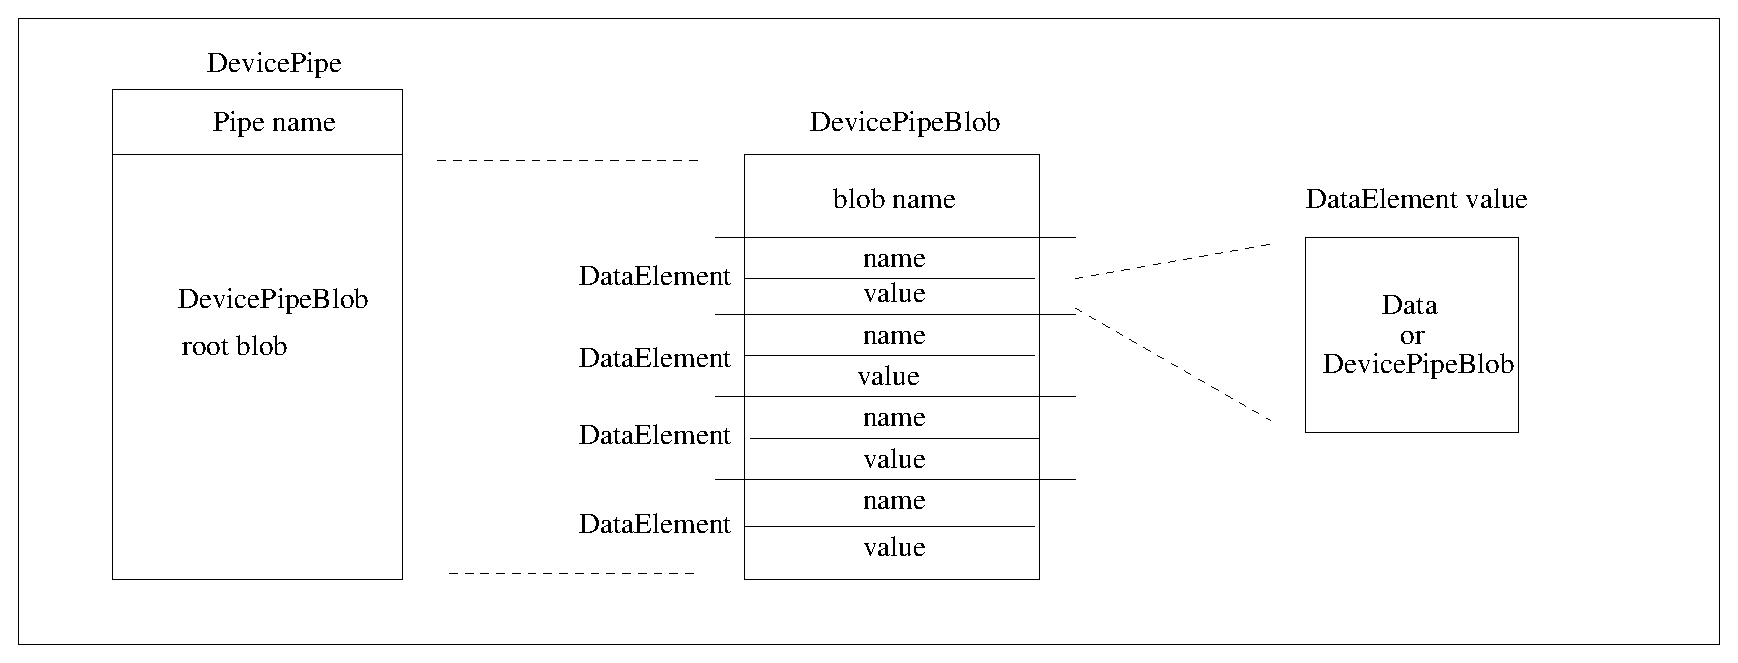
\includegraphics[width=14cm,height=8cm]{gen_api/pipe}
\par\end{centering}

\protect\caption{DevicePipe data structure}
\label{ }
\end{figure}


Many methods to insert/extract data into/from a DevicePipe are available.
In the DevicePipe class, these methods simply forward their action
to the DevicePipe root blob. The same methods are available in the
DevicePipeBlob in case you need to use the recursivity provided by
this data structure.


\subsection{Reading a pipe}

When you read a pipe, you have to extract data received from the pipe.
Because data transferred through a pipe can change at any moment,
two differents cases are possible:
\begin{enumerate}
\item The client has a prior knowledge of what should be transferred through
the pipe
\item The client does not know at all what has been received through the
pipe
\end{enumerate}
Those two cases are detailed in the following sub-chapters.


\subsubsection{Extracting data with pipe content prior knowledge}

To extract data from a DevicePipe object (or from a DevicePipeBlob
object), you have to use its extraction operator \textquotedbl{}>\textcompwordmark{}>\textquotedbl{}.
Let's suppose that we already know (prior knowledge) that the pipe
contains 3 data elements with a Tango long, an array of double and
finally an array of unsigned short. The code you need to extract these
data is (Without error case treatment detailed in a next sub-chapter)


\begin{minted}[linenos]{cpp}
1 DevicePipe dp = mydev.read_pipe("MyPipe");
2 
3 DevLong dl;  
4 vector<double> v_db;  
5 DevVarUShortArray *dvush = new DevVarUShortArray();
6 
7 dp >> dl >> v_db >> dvush;
8
9 delete dvush;
\end{minted}


The pipe is read at line 1. Pipe (or root blob) data extracttion is
at line 7. As you can see, it is just a matter of chaining extraction
operator (\textquotedbl{}>\textcompwordmark{}>\textquotedbl{}) into
local data (declared line 3 to 5). In this example, the transported
array of double is extracted into a C++ vector while the unsigned
short array is extracted in a Tango sequence data type. When you extract
data into a vector, there is a unavoidable memory copy between the
DevicePipe object and the vector. When you extract data in a Tango
sequence data type, there is no memory copy but the extraction method
consumes the memory and it is therefore caller responsability to delete
the memory. This is the rule of line 9. If there is a DevicePipeBlob
inside the DevicePipe, simply extract it into one instance of the
DevicePipeBlob class.

You may notice that the pipe root blob data elements name are lost
in the previous example. The Tango API also has a DataElement\index{DataElement}
class which allows you to retrieve/set data element name. The following
code is how you can extract pipe data and retrieve data element name
(same pipe then previously)


\begin{minted}[linenos]{cpp}
1 DevicePipe dp = mydev.read_pipe("MyPipe");
2 
3 DataElement<DevLong> de_dl;  
4 DataElement<vector<double> > de_v_db;  
5 DataElement<DevVarUShortArray *> de_dvush(new DevVarUShortArray());
6 
7 dp >> de_dl >> de_v_db >> de_dvush;
8
9 delete de_dvush.value;
\end{minted}


The extraction line (number 7) is similar to the previous case but
local data are instances of DataElement class. This is template class
and instances are created at lines 4 to 6. Each DataElement instance
has only two elements which are:
\begin{enumerate}
\item The data element name (a C++ string): \emph{name}
\item The data element value (One instance of the template parameter): \emph{value}
\end{enumerate}

\subsubsection{Extracting data in a generic way (without prior knowledge)}

Due to the dynamicity of the data transferred through a pipe, the
API alows to extract data from a pipe without any prior knowledge
of its content. This is achived with methods \emph{get\_data\_elt\_nb()},
\emph{get\_data\_elt\_type()}, \emph{get\_data\_elt\_name()} and the
extraction operator \textquotedbl{}>\textcompwordmark{}>\textquotedbl{}.
These methods belong to the DevicePipeBlob class but they also exist
on the DevicePipe class for its root blob. Here is one example of
how you use them:


\begin{minted}[linenos]{cpp}
1  DevicePipe dp = mydev.read_pipe("MyPipe");
2
3  size_t nb_de = dp.get_data_elt_nb();  
4  for (size_t loop = 0;loop < nb;loop++)
5  {      
6     int data_type = dp.get_data_elt_type(loop);      
7     string de_name = dp.get_data_elt_name(loop);      
8     switch(data_type)      
9     {         
10        case DEV_LONG:         
11        {             
12            DevLong lg;             
13            dp >> lg;         
14        }         
15        break;
16        
17        case DEVVAR_DOUBLEARRAY:         
18        {             
19            vector<double> v_db;             
20            dp >> v_db;         
21        }         
22        break;         
23        ....      
24    }  
25    ...  
26 }
\end{minted}


The number of data element in the pipe root blob is retrieve at line
3. Then a loop for each data element is coded. For each data element,
its value data type and its name are retrieved at lines 6 and 7. Then,
according to the data element value data type, the data are extracted
using the classical extraction operator (lines 13 or 20)


\subsubsection{Error management}

By default, in case of error, the DevicePipe object throws different
kind of exceptions according to the error kind. It is possible to
disable exception throwing. If you do so, the code has to test the
DevicePipe state after extraction. The possible error cases are:
\begin{itemize}
\item DevicePipe object is empty
\item Wrong data type for extraction (For instance extraction into a double
data while the DataElement contains a string)
\item Wrong number of DataElement (Extraction code extract 5 data element
while the pipe contains only four)
\item Mix of extraction (or insertion) method kind (classical operators
<\textcompwordmark{}< or >\textcompwordmark{}>) and {[}{]} operator.
\end{itemize}
Methods \emph{exceptions()} and \emph{reset\_exceptions()} of the
DevicePipe and DevicePipeBlob classes allow the user to select which
kind of error he is interested in. For error treatment without exceptions,
methods \emph{has\_failed()} and \emph{state()} has to be used. See
reference documentation for details about these methods.


\subsection{Writing a pipe}

Writing data into a DevicePipe or a DevicePipeBlob is similar to reading
data from a pipe. The main method is the insertion operator \textquotedbl{}<\textcompwordmark{}<\textquotedbl{}.
Let's have a look at a first example if you want to write a pipe with
a Tango long, a vector of double and finally an array of unsigned
short.


\begin{minted}[linenos]{cpp}
1  DevicePipe dp("MyPipe");
2 
3  vector<string> de_names {"FirstDE","SecondDE","ThirdDE"};
4  db.set_data_elt_names(de_names);
5
6  DevLong dl = 666;  
7  vector<double> v_db {1.11,2.22};
8  unsigned short *array = new unsigned short [100];
9  DevVarUShortArray *dvush = create_DevVarUShortArray(array,100);
10
11 try  
12 {     
12    dp << dl << v_db << dvush;
13    mydev.write_pipe(dp);
14 }
15 catch (DevFailed &e)
16 {     
17    cout << "DevicePipeBlob insertion failed" << endl;     
18    ....  
19 }
\end{minted}


Insertion into the DevicePipe is done at line 12 with the insert operators.
The main difference with extracting data from the pipe is at line
3 and 4. When inserting data into a pipe, you need to FIRST define
its number od name of data elements. In our example, the device pipe
is initialized to carry three data element and the names of these
data elements is defined at line 4. This is a mandatory requirement.
If you don't define data element number, exception will be thrown
during the use of insertion methods. The population of the array used
for the third pipe data element is not represented here.

It's also possible to use DataElement class instances to set the pipe
data element. Here is the previous example modified to use DataElement
class.


\begin{minted}[linenos]{cpp}
1  DevicePipe dp("MyPipe");
2
3  DataElement<DevLong> de_dl("FirstElt",666);  
4  vector<double>  v_db {1.11,2.22};
5  DataElement<vector<double> > de_v_db("SecondElt,v_db);
6
7  unsigned short *array = new unsigned short [100];
8  DevVarUShortArray *dvush = create_DevVarUShortArray(array,100);
9  DataElement<DevVarUShortArray *> de_dvush("ThirdDE",array);
10
11 try  
12 {     
12    dp << de_dl << de_v_db << de_dvush;
13    mydev.write_pipe(dp);
14 }
15 catch (DevFailed &e)
16 {     
17    cout << "DevicePipeBlob insertion failed" << endl;     
18    ....  
19 }
\end{minted}


The population of the array used for the third pipe data element is
not represented here. Finally, there is a third way to insert data
into a device pipe. You have to defined number and names of the data
element within the pipe (similar to first insertion method) but you
are able to insert data into the data element in any order using the
\textquotedbl{}{[}{]}\textquotedbl{} operator overwritten for the
DevicePipe and DevicePipeBlob classes. Look at the following example:


\begin{minted}[linenos]{cpp}
1  DevicePipe dp("MyPipe");
2 
3  vector<string> de_names {"FirstDE","SecondDE","ThirdDE"};
4  db.set_data_elt_names(de_names);
5
6  DevLong dl = 666;  
7  vector<double> v_db = {1.11,2.22};
8  unsigned short *array = new unsigned short [100];
9  DevVarUShortArray *dvush = create_DevVarUShortArray(array,100);
10
11 dp["SecondDE"] << v_db;
12 dp["FirstDE"] << dl;
13 dp["ThirdDE"] << dvush;
\end{minted}


Insertion into the device pipe is now done at lines 11 to 13. The
population of the array used for the third pipe data element is not
represented here. Note that the data element name is case insensitive.


\subsubsection{Error management}

When inserting data into a DevicePipe or a DevicePipeBlob, error management
is very similar to reading data from from a DevicePipe or a DevicePipeBlob.
The difference is that there is one moer case which could trigger
one exception during the insertion. This case is
\begin{itemize}
\item Insertion into the DevicePipe (or DevicePipeBlob) if its data element
number have not been set.
\end{itemize}

\section{Device locking\index{Locking}}

Starting with Tango release 7 (and device inheriting from Device\_4Impl),
device locking is supported. For instance, this feature could be used
by an application doing a scan on a synchrotron beam line. In such
a case, you want to move an actuator then read a sensor, move the
actuator again, read the sensor...You don't want the actuator to be
moved by another client while the application is doing the scan. If
the application doing the scan locks the actuator device, it will
be sure that this device is \textquotedbl{}reserved\textquotedbl{}
for the application doing the scan and other client will not be able
to move it until the scan application un-locks this actuator.

A locked device is protected against:
\begin{itemize}
\item \emph{command\_inout} call except for device state and status requested
via command and for the set of commands defined as allowed following
the definition of allowed command in the Tango control access schema.
\item \emph{write\_attribute} and \emph{write\_pipe} call
\item \emph{write\_read\_attribute, write\_read\_attributes} and \emph{write\_read\_pipe}
call
\item \emph{set\_attribute\_config }and\emph{ set\_pipe\_config} call
\item polling and logging commands related to the locked device
\end{itemize}
Other clients trying to do one of these calls on a locked device will
get a DevFailed exception. In case of application with locked device
crashed, the lock will be automatically release after a defined interval.
The API provides a set of methods for application code to lock/unlock
device. These methods are:
\begin{itemize}
\item \emph{DeviceProxy::lock()} and \emph{DeviceProxy::unlock()} to lock/unlock
device
\item \emph{DeviceProxy::locking\_status()}, \emph{DeviceProxy::is\_locked()},
\emph{DeviceProxy::is\_locked\_by\_me()} and \emph{DeviceProxy::get\_locker()}
to get locking information
\end{itemize}
These methods are precisely described in the API reference chapters.


\section{Reconnection\index{reconnection} and exception}

The Tango API automatically manages re-connection between client and
server in case of communication error during a network access between
a client and a server. By default, when a communication error occurs,
an exception is returned to the caller and the connection is internally
marked as bad. On the next try to contact the device, the API will
try to re-build the network connection. With the \emph{set\_transparency\_reconnection\index{set-transparency-reconnection}()}
method of the DeviceProxy\index{DeviceProxy} class, it is even possible
not to have any exception thrown in case of communication error. The
API will try to re-build the network connection as soon as it is detected
as bad. This is the default mode. See \ref{sec:Reconnection-and-exception}
for more details on this subject.


\section{Thread\index{thread} safety}

Starting with Tango 7.2, some classes of the C++ API has been made
thread safe. These classes are:
\begin{itemize}
\item DeviceProxy
\item Database
\item Group
\item ApiUtil
\item AttributeProxy
\end{itemize}
This means that it is possible to share between threads a pointer
to a DeviceProxy instance. It is safe to execute a call on this DeviceProxy
instance while another thread is also doing a call to the same DeviceProxy
instance. Obviously, this also means that it is possible to create
thread local DeviceProxy instances and to execute method calls on
these instances. Nevertheless, data local to a DeviceProxy instance
like its timeout are not managed on a per thread basis. For a DeviceProxy
instance shared between two threads, if thread 1 changes the instance
timeout, thread 2 will also see this change.


\section{Compiling and linking a Tango client}

Compiling and linking a Tango client is similar to compiling and linking
a Tango device server. Please, refer to chapter \textquotedbl{}Compiling,
Linking and executing a Tango device server process\textquotedbl{}
(\ref{sec:Compiling,-linking-and}) to get all the details.

\begin{center}

\label{ThreeRicardo}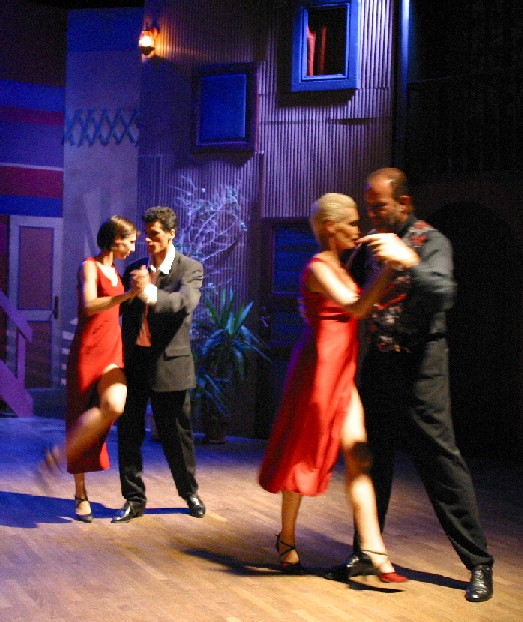
\includegraphics[scale=2]{dance/0066-reduc}

\end{center}
